%-----------------------------------------
% Note: Use pdflatex to process this file.
%-----------------------------------------

%\documentclass{article}
\documentclass{hitec}
\usepackage{color,soul}

\usepackage{setspace}
\usepackage{graphicx}
\usepackage{moreverb}    % Defines {listing} environment.
\usepackage{amsmath, amsthm, amssymb, amsbsy, mathtools}
\usepackage{alltt}
\usepackage{rotating}
\usepackage{subcaption}
\usepackage{toc-bmad}
\usepackage{xspace}
\usepackage[section]{placeins}   % For preventing floats from floating to end of chapter.
\usepackage{longtable}   % For splitting long vertical tables into pieces
\usepackage{index}
\usepackage{multirow}
\usepackage{booktabs}    % For table layouts
\usepackage{yhmath}      % For widehat
\usepackage{xcolor}      % Needed for listings package.
\usepackage{listings}
\usepackage[T1]{fontenc}   % so _, <, and > print correctly in text.
\usepackage[strings]{underscore}    % to use "_" in text
\usepackage[pdftex,colorlinks=true,bookmarksnumbered=true]{hyperref}   % Must be last package!

\definecolor{light-gray}{gray}{0.95}
\lstset{backgroundcolor=\color{light-gray}}
\lstset{xleftmargin=0cm}
\lstset{framexleftmargin=0.3em}
%\lstset{basicstyle = \ttfamily\fontsize{11}{11}\selectfont} 
\lstset{basicstyle = \small}
\lstnewenvironment{code}{}{}

%---------------------------------------------------------------------------------

\definecolor{lightestgray}{gray}{0.99}
\sethlcolor{lightestgray}
\soulregister{\texttt}{1}
\newcommand\dottcmd[1]{\hl{\em#1}\endgroup}
%\newcommand\dottcmd[1]{{#1}\endgroup}
\newcommand{\vn}{\begingroup\catcode`\_=11 \catcode`\%=11 \dottcmd}
\newcommand{\da}{\vn{dynamic_aperture}\xspace}
\newcommand{\Newline}{\hfil \\}
\newcommand{\sref}[1]{$\S$\ref{#1}}
\newcommand{\Th}{$^{th}$\xspace}
\newcommand{\ltt}{\vn{long_term_tracking}\xspace}

%---------------------------------------------------------------------------------

\renewcommand{\textfraction}{0.1}
\renewcommand{\topfraction}{1.0}
\renewcommand{\bottomfraction}{1.0}

\settextfraction{0.9}  % Width of text
\setlength{\parindent}{0pt}
\setlength{\parskip}{1ex}
%\setlength{\textwidth}{6in}
\newcommand{\Section}[1]{\section{#1}\vspace*{-1ex}}

\newenvironment{display}
  {\vspace*{-1.5ex} \begin{alltt}}
  {\end{alltt} \vspace*{-1.0ex}}

%---------------------------------------------------------------------------------

\title{Dynamic_Aperture Program}
\author{}
\date{David Sagan \\ September 24, 2022}

\begin{document}
\pdfbookmark[1]{Contents}{contents}

\maketitle

\tableofcontents

%---------------------------------------------------------------------------------
\Section{Introduction} 
\label{s:intro}

The \da program is for measuring the dynamic aperture. The concept of \vn{dynamic aperture} is that
a particle reaching a certain amplitude will quickly be resonantly driven to large amplitude where
it is lost. This amplitude where the particle becomes unstable is the dynamic aperture. This is to
be contrasted by the \vn{physical aperture} which is the aperture where a particle strikes the wall
of the beam chamber. The general idea in designing lattices is to make sure that the dynamic
aperture is large enough so that, in the normal course of events, particles in the beam have a very
small probability of getting lost due to their amplitude exceeding the dynamic aperture. For long
term stability, a common rule of thumb is to design lattices such that the dynamic aperture is 10 times
the beam sigma.\footnote
  {
While this might seem excessive, this rule of thumb gives some safety margin which is desirable
since designs are never exact.
  }
For injection studies, the minimum dynamic aperture will be determined in part by the size of the
injected beam. In any case, if the dynamic aperture is larger than the physical aperture, increasing
the dynamic aperture further will not help beam stability. 

If there are no apertures set in lattice used by the \da program, the calculated aperture will be the
dynamic aperture. If apertures are set in the lattice, the calculated aperture will be the minimum of
the dynamic and physical apertures.

The \da program is built atop the Bmad software toolkit \cite{b:bmad}. The Bmad toolkit is a
library, developed at Cornell, for the modeling relativistic charged particles in storage rings and
Linacs, as well as modeling photons in x-ray beam lines.

For historical reasons, the \vn{Tao} program (another Bmad based program) is also capable of
calculating the dynamic aperture.  In fact both programs use the same underlying code for the
aperture analysis. The basic difference is that the \da program is more flexible in terms of
tracking. For example, the \da program can handle \vn{ramper} elements and track with maps.

%------------------------------------------------------------------
\Section{Running the Dynamic Aperture Program} 
\label{s:run}

The \da program comes with the ``Bmad Distribution'' which is a package which contains the Bmad toolkit
library along with a number of Bmad based programs. See the Bmad web site for more details.

If the Bmad Distribution is compiled with \vn{OpenMP} enabled (see the documentation on the Bmad
Distribution ``Off-Site'' setup for more details), the \da program can be run parallel. With OpenMP
the computation load is distributed over a number of cores on the machine you are using. To set the
number of cores set the \vn{OMP_NUM_THREADS} environment variable. Example:
\begin{code}
export OMP_NUM_THREADS=8
\end{code}
And run the program as normal as detailed below.

See the documentation for setting up the Bmad environment variables at
\begin{code}
  https://wiki.classe.cornell.edu/ACC/ACL/RunningPrograms
\end{code}

Once the Bmad environment variables have been set, the syntax for invoking the program is:
\begin{code}
  dynamic_aperture {<master_input_file_name>}
\end{code}
Example:
\begin{code}
  dynamic_aperture my_input_file.init
\end{code}
The \vn{<master_input_file_name>} optional argument is used to set the master input file name. The
default value is ``\vn{dynamic_aperture.init}''. The syntax of the master input file is explained
in \sref{s:input}.

Example input files are in the directory (relative to the root of a Distribution):
\begin{code}
  bsim/dynamic_aperture/example
\end{code}

%------------------------------------------------------------------
\Section{Time Ramping --- Time Varying Element Parameters}
\label{s:ramp}

``\vn{Ramping}'' is the situation where lattice parameters are changing as a function of time over
many turns. Ramping examples include changing magnet and RF strengths to ramp the beam energy or
changing magnet strengths to squeeze beta at the interaction pont of a colliding beam machine.

Ramping is accomplished by defining \vn{ramper} elements in the lattice file and setting
\vn{ramping_on} to True in the master input file (\sref{s:input}). Ramper elements will be applied
to each lattice element in turn before particles are tracked through them. See the Bmad manual for
documentation on \vn{ramper} syntax.

Example:
\begin{code}
  ramp_e: ramper = \{*[e_tot]:\{4e+08, 4.00532e+08, 4.01982e+08, ...\}\},
                var = \{time\}, x_knot = \{0, 0.001, 0.002, ...\}

  amp = 1e9;  omega = 0.167;  t0 = 0.053
  ramp_rf: ramper = \{rfcavity::*[voltage]:amp*sin(omega *(time + t0)),
        rfcavity::*[phi0]:0.00158*time^2 + 2*q \}, var = \{time, q\}
\end{code}
The ``\vn{*[e_tot]}'' construct in the definition of \vn{ramp_e} means that the ramper will be
applied all elements (since the wild card character ``\vn{*}'' will match to any element name), and
it is the element's \vn{e_tot} attribute (the element's reference energy) that will be varied.

In the above example, the \vn{ramp_rf} ramper will be applied to all \vn{rfcavity} elements with
the cavity voltage and phase (\vn{phi0}) being varied.

Important restriction: Only those
ramper elements that have \vn{time} as the first variable will be used and it will be this variable
that is varied over time. 

In the case where the reference energy \vn{e_tot} or reference momentum \vn{p0c} is being varied, the
effect on an element will depend upon the setting of the element's \vn{field_master} parameter. For
example:
\begin{code}
  q1: quadrupole, k1 = 0.3
  q2: quadrupole, k1 = 0.3, field_master = T
\end{code}
In this example, \vn{q1} will have its \vn{field_master} parameter set to \vn{False} since the
quadrupole strength was specified using the normalized strength \vn{k1}. With \vn{q1}, since
\vn{field_master} is False, varying the reference energy or momentum will result in the normalized
strength \vn{k1} remaining fixed and the unnormalized strength \vn{B1_gradient} varying in
proportion to the reference momentum. With \vn{q2}, since \vn{field_master} is True, the
unnormalized strength \vn{B1_gradient} will remain fixed and normalized \vn{k1} will vary
inversely with the reference momentum.

Before a simulation, individual ramper elements may be toggled on or off by setting the element's
\vn{is_on} attribute in the lattice file: 
\begin{code}
  ramp_rf: ramper = ...  ! Ramper element defined.
  ramp_rf[is_on] = F     ! Ramper element turned off.
\end{code}

%------------------------------------------------------------------
\Section{Fortran Namelist Input}
\label{s:namelist}

Fortran namelist syntax is used for parameter input in the master input file. The general form of a namelist is
\begin{code}
&<namelist_name>
  <var1> = ...
  <var2> = ...
  ...
/
\end{code}
The tag \vn{"\&<namelist_name>"} starts the namelist where \vn{<namelist_name>} is the name of the
namelist. The namelist ends with the slash \vn{"/"} tag. Anything outside of this is ignored. Within
the namelist, anything after an exclamation mark \vn{"!"} is ignored including the exclamation
mark. \vn{<var1>}, \vn{<var2>}, etc. are variable names. Example:
\begin{code}
&place 
  section = 0.0, "arc_std", "elliptical", 0.045, 0.025 
/
\end{code}
here \vn{place} is the namelist name and \vn{section} is a variable name.  Notice that here
\vn{section} is a ``structure'' which has five components -- a real number, followed by two strings,
followed by two real numbers.

Everything is case insensitive except for quoted strings.

Logical values are specified by \vn{True} or \vn{False} or can be abbreviated \vn{T} or
\vn{F}. Avoid using the dots (periods) that one needs in Fortran code.

\clearpage

\begin{figure}[tb]
  \centering
  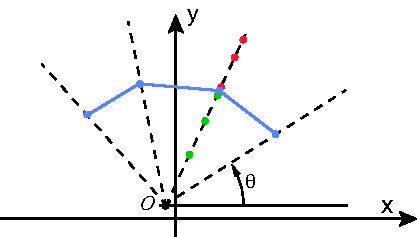
\includegraphics[width=4in]{aperture-rays.pdf}
  \caption{
The calculation of a dynamic aperture curve in the $x$-$y$ plane at a given initial $p_z$ value
involves calculating aperture curve points (blue dots) along a set of ``rays'' (dashed lines) having
a common origin point ($\cal O$) which is taken to be the reference orbit. The line segments between
points is simply for visualization purposes. The calculation of an aperture curve point along a
given ray involves iteratively tracking particles with different starting $(x, y)$ position values
to find the boundary between stable (green dots) and unstable (red dots) motion.
  }
  \label{f:da-ray}
\end{figure}

%------------------------------------------------------------------
\Section{Master Input File}
\label{s:input}

The \vn{master input file} holds the parameters needed for running the \da program. The master input
file must contain a single namelist (\sref{s:namelist}) named \vn{params}.  Example:
\begin{code}
&params
  dat_file = "da.dat"

  ltt%lat_file           = "lat.bmad"     ! Bmad lattice file
  ltt%ramping_on         = False
  ltt%ramping_start_time = 0
  ltt%rfcavity_on        = True
  ltt%tracking_method    = "BMAD"
  ltt%ele_start          = ""
  ltt%map_order          = 5
  ltt%random_seed        = 0
  ltt%ptc_aperture       = 0.1, 0.1
  ltt%exclude_from_maps  = "beambeam::*"
  ltt%symplectic_map_tracking = False
  ltt%set_beambeam_z_crossing = False
  ltt%use_rf_clock       = F

  bmad_com%radiation_damping_on = F
  bmad_com%radiation_fluctuations_on = F 

  dpz = 0.000, 0.005, 0.010
  da_param%min_angle = 0
  da_param%max_angle = 3.1415926
  da_param%n_angle = 0
  da_param%n_turn = 2000
  da_param%x_init = 1e-3
  da_param%y_init = 1e-3
  da_param%rel_accuracy = 1e-2
  da_param%abs_accuracy = 1e-5
/
\end{code}
Note: The parameters beginning with ``\vn{ltt}'' are parameters that are common with the
\ltt program. The parameters beginning with ``\vn{da_param}'' are parameters
that are common with the dynamic aperture tracking in the Tao program

The parameters in the master input file are:
\begin{description}
%
\item[bmad_com\%...] \Newline
The \vn{bmad_com} structure contains various parameters that affect tracking. For example, whether
radiation damping is included in tracking. A full list of \vn{bmad_com} parameters is detailed in
the Bmad reference manual. Note: \vn{bmad_com} parameters can be set in the Bmad lattice file as
well. \vn{Bmad_com} parameter set in the master input file will take precedence over parameters set
in the lattice file.
%
\item[da_param\%n_turn] \Newline
Number of turns to track. 
%
\item[da_param\%n_angle] \Newline
The number of boundary points calculated for a scan is set by the \vn{da_param%n_angle} parameter. 
%
\item[da_param\%min_angle, da_param\%max_angle] \Newline
These parameters set the ray minimum and maximum angles, labeled $\theta$ in Fig~\ref{f:da-ray}, in a
scan. In the example above the angle ranges from 0 to $pi$.  That is, the upper half-plane. These
are typical settings since typically storage rings are vertically symmetric so the aperture curves
should vertically symmetric as well.

The angles between adjacent rays is not uniform but are rather calculated to give a roughly
equal spacing between boundary points. This is done by looking at the aperture
points on a horizontal and a vertical ray and then scaling the ray angles appropriately).
%
\item[da_param\%rel_accuracy, da_param\%abs_accuracy] \Newline
These parameters set the relative and absolute accuracies that determine when the search for a
boundary point is considered accurate enough.

If $r = \sqrt{(x-x_0)^2 + (y-y_0)^2}$ is the distance
along any ray of the computed boundary point, where $(x_0, y_0)$ are the coordinates of the origin
point, the search for the boundary point will stop then the accuracy of the boundary point is below
the desired accuracy $\sigma_{cut}$ which is computed from
\begin{equation}
  \sigma_{cut} = \sigma_a + r \, \sigma_r
\end{equation}
with $\sigma_a$ begin the absolute accuracy and $\sigma_r$ being the relative accuracy.
%
\item[da_param\%x_init, da_param\%y_init] \Newline
These parameters set the initial $x$ and $y$ values used in the first two boundary point searches.
The values of these parameters will not affect significantly affect the computed curve but will
affect the computation time. If not set, these parameters will default to 0.001 meter.
%
\item[dat_file] \Newline
Name of the data output file. This name is required.
%
\item[dpz] \Newline
The \vn{dpz} parameter array is a list of $p_z$ values to use. The number of scans (dynamic aperture curves)
that are produced is equal to the number of \vn{pz} values.


%
\item[ele_start] \Newline
Name or element index of the element to start the tracking. Examples:
\begin{code}
  ele_start = "Q3##2"   ! 2nd element named Q3 in the lattice.
  ele_start = 37        ! 37th element in the lattice.
\end{code}
The default is to start at the beginning of the lattice. Notice that the tracking starts at the
downstream end of the element so the first element tracked through is the element after the chosen
one.
%
\item[ltt\%ele_start] \Newline
Name or element index of the element to start the tracking. Examples:
\begin{code}
ele_start = "Q3##2"   ! 2nd element named Q3 in the lattice.
ele_start = 37        ! 37th element in the lattice.
\end{code}
The default is to start at the beginning of the lattice. Notice that the tracking starts at the
downstream end of the element so the first element tracked through is the element after the chosen
one. Also see \vn{ltt%ele_stop}.
%
\item[ltt\%exclude_from_maps] \Newline
List of elements to exclude when constructing maps for \vn{SLICK} tracking. These elements will be
individually tracking. The default value is \vn{"beambeam::*"} which excludes any \vn{beambeam}
element. See the Bmad manual section on ``\vn{Matching to Lattice Element Names}'' for details on
the format for such lists.
%
\item[ltt\%lat_file] \Newline
Name of the Bmad lattice file to use. This name is required. Note: In an old, deprecated format this parameter
was called \vn{lat_file}.
%
\item[ltt\%map_order] \Newline
Map order. See Section~\sref{s:track.methods}. The default is what is set in the lattice
file and if not set in the lattice file the default is 3. Note: \vn{ltt%map_order} is only used when
generating a map.  When a map is read in from a file, the order of this map is independent of the
current setting of \vn{ltt%map_order}.
%
\item[ltt\%ptc_aperture] \Newline
The PTC code does not have apertures. This being the case, for \vn{ltt%tracking_method} set to
\vn{"MAP"} or \vn{"PTC"}, \vn{ltt%ptc_aperture}, which is a 2-vector, defines \vn{x} and \vn{y}
apertures. The default is 0.1~meter in both the horizontal and vertical. When used, the aperture is
applied at the beginning/end of the lattice. PTC has an internal aperture of 1.0~meter. To be safe,
the \ltt program will additionally impose a 0.9~meters aperture independent of the setting of
\vn{ltt%ptc_aperture}.
%
\item[ltt\%ramping_on] \Newline
If set to True, \vn{ramper} control elements will be use to modify the lattice during tracking
(\sref{s:ramp}). Default is False. Note: In an old, deprecated format this parameter
was called \vn{ramping_on}.
%
\item[ltt\%ramping_start_time] \Newline
The starting (offset) time used to set \vn{ramper} elements. This enables simulations to start in the middle
of a ramp cycle. Default is 0.
%
\item[ltt\%random_seed] \Newline
The random number seed used by the random number generator. If set to 0, the
system clock will be used. That is, if set to 0, the output results will vary from run to run.
%
\item[ltt\%rfcavity_on] \Newline
If set to \vn{False}, the voltage on all RF cavity elements will be turned off. Default is
\vn{True}.  Note: In an old, deprecated format the corresponding parameter was called
\vn{set_rf_off}.
%
\item[ltt\%set_beambeam_z_crossing] \Newline
If True (default is false), set the \vn{z_crossing} parameter of any \vn{beambeam} element in the
lattice to the phase space $z$ value of the closed orbit? See the Bmad manual for a discussion of
the \vn{z_crossing} parameter. Generally, \vn{ltt%set_beambeam_z_crossing} should be set True.
%
\item[ltt\%symplectic_map_tracking]\Newline
If False (the default), the maps used for tracking will be a set of truncated Taylor series
polynomials. If True, the tracking maps will be derived from the Taylor map by partially inverting
it forming an implicit symplectic map. The advantage of the symplectic map is that it is symplectic.
The disadvantage is that, being an implicit map, the computation time will be longer.
%
\item[ltt\%use_rf_clock] \Newline
The \vn{ltt%use_rf_clock} logical is only relavent if Bmad tracking is being used in conjunction with
absolute time tracking and the discussion here assumes Bmad tracking with absolute time tracking.\footnote
  {
See the Bmad manual for a discussion of absolute versus relative time tracking.
  }
If \vn{ltt%use_rf_clock} is set to False (the default), the time used to calculate the phase of any
varying fields is the absolute time which increases turn-by-turn. Over many turns this may lead to
round-off error. For example, with a 10~GHz cavity, if the phase needs to be measured to one part in
$10^5$, it will not be possible to run a simulation past 10~seconds since the double precision
numbers used in the code have an accuracy of $10^{-16}$. 

There are several possible ways to avoid this round-off problem. If all the frequencies of all the time
varying fields are commensurate with the length of the lattice, relative time tracking can be used
which uses the particle's $z$ phase space coordinate as the effective clock.\footnote
  {
Note: Absolute time tracking is not available with PTC. That is, any PTC based tracking is relative
time tracking.
  }
If all frequencies are commensurate with each other, but are not commensurate with the lattice
length, time patches (patch elements that shift the reference time) can be used with relative time
tracking.  Finally, if all the frequencies are commensurate, the ``\vn{RF clock}'' can be used with
absolute time tracking by setting \vn{ltt%use_rf_clock} to True. The RF clock is simply a clock whose
time is reset periodically to be in the range $[0, t_{rf}]$ where $t_{rf}$ is a time period chosen by
Bmad to be commensurate with the frequencies of the time varying fields.\footnote
  {
If not all the frequencies are commensurate, Bmad will make a best choice and the fields that have
frequencies that are not commensurate with the RF clock will use the standard clock instead.
  }
\end{description}

%------------------------------------------------------------------
\Section{Tracking Methods}
\label{s:track.methods}

The setting of the
parameter \vn{ltt%tracking_method} determines how particles are tracked. Possible settings are:
\begin{code}
"MAP"     ! Tracking using maps.
"PTC"     ! Element-by-element tracking with PTC. Slow.
"BMAD"    ! Element-by-element tracking using Bmad. Default. Slow.
\end{code}

which is used to determine if tracking is done using a map or not. If a map is used, the order of
the map (the degree at which the Taylor series comprising the map are truncated) is given by
\vn{ltt%map_order} parameter. A larger map order will mean better accuracy at the expense of more
computation time. Tracking using a map will be extremely quick compared to element-by-element
tracking. However, map tracking can be inaccurate if the map order is too small or the particle
amplitude is too large.

Only the \vn{BMAD} method is able to handle a machine that is being ramped (\sref{s:ramp}). That is,
when \vn{ltt%ramping_on} set to True. The program will detect if there is a conflict and issue an error
message and stop.

%------------------------------------------------------------------
\Section{Map Tracking}
\label{s:map}

The \ltt program uses the PTC/FPP library of \'Etienne Forest to handle Taylor maps which can be
constructed to any arbitrary order. In particular, PTC is used for constructing the map(s) used for
tracking when the \vn{ltt%tracking_method} parameter is set to "\vn{MAP}" (\sref{s:sim.params}). PTC
tracking is also used when \vn{ltt%tracking_method} is set to "\vn{PTC}". In this case, tracking is
done element-by-element using symplectic integration.

Note: Using maps is not compatible when a machine is being ramped (\sref{s:ramp}).

Sometimes it is convenient to exclude certain lattice elements from a map. For example, the
beam-beam interaction is highly non-linear so excluding any \vn{beambeam} elements can improve map
accuracy at larger amplitudes. Which elements are excluded is determined by the setting of
\vn{ltt%exclude_from_maps} which is a list of what elements are to be excluded. Elements can be
excluded for a number of reasons. When an element is excluded, multiple maps are created, one for
each of the sections of the lattice where there are no excluded elements. In this case, tracking
consists of using a map to track from one excluded element to the next followed by tracking through
the excluded element.

{\em Important!} Maps cannot model RF elements that have a frequency not commensurate with the
one-turn frequency. The reason for this is that a map is just a function that maps the particle's
starting phase space coordinates to the particle's ending coordinates independent of how many turns
the particle has been tracked. But if an RF element has a frequency not commensurate with the
one-turn frequency the kick given a particle going through the element will depend upon the turn
index. Maps can be used to model a lattice with such RF elements, but in this case such elements
must be excluded from be incorporated in any map by setting \vn{ltt%exclude_from_maps} appropriately.

Depending upon how things are setup, a \vn{PTC} map can include radiation damping and fluctuations
effects. \footnote
  {
Radiation fluctuations are included by actually using two maps to track a particle from one point to
the next. One map represents the transport with damping and the second map represents the
fluctuations. When a particle is tracked, the first map with damping is applied and then the second
map is applied using six random numbers.
  }
Damping and excitation are controlled by two parameters that can be set in the master input file:
\begin{code}
bmad_com%radiation_damping_on
bmad_com%radiation_fluctuations_on
\end{code}

Maps are saved to a file for use if the program is rerun. For linear maps, an ASCII file
can be produced by setting \vn{ltt%map_ascii_output_file}.

%------------------------------------------------------------------
\Section{Tuning Map and PTC Tracking Parameters}
\label{s:map.tuning}

When tracking using maps or element-by-element with PTC there are a few points to keep in
mind. First is that \vn{PTC} tracks through a lattice element step by step. This is true for both
map creation and symplectic integration. This means that the setting of the element parameter
\vn{integrator_order}\footnote
  {
Note: Valid settings for \vn{integrator_order} are 2, 4, and 6
  }
or \vn{num_steps} (or \vn{ds_step}) for each element will affect the accuracy and speed of the
computations. Bmad tries to choose reasonable default settings for the integrator order and number
of steps however the calculation is not perfect. To make sure that the integrator order and number
of steps is set properly, vary both and choose values (which can be different for different
elements) such that the number of steps and integrator order is minimal (to minimize computation
time) while at the same time is large enough so that results do not change significantly if the
number of steps or is varied. Generally it is much better to use a large integrator order and a
small step size rather than vice versa with the proviso that for elements with a longitudinally
varying field (think wigglers or undulators), the step size must be small compared to the typical
longitudinal length scale over which the field is varying (this length scale is the pole period
length with with wigglers and undulators).

Another thing to keep in mind is that whether a map will give accurate results is dependent on a
number of factors. One factor is the order of the map. Generally higher order is better but will
take more computation time. When the lattice is tracked using a single map, the tracking is only
valid when the tracked particles are far from any strong resonances. That is, if you are interested
in tracking halo particles, you probably should not be using a single map.

In terms of speed, using maps will be the fastest, using standard Bmad tracking will be much
slower, and using PTC element-by-element tracking will be slowest.

In terms of symplecticity, both the PTC tracking and map tracking will be symplectic.
Bmad is not symplectic but the deviation from symplecticity is generally fairly small. If the
radiation effects are large enough, the radiative stochastic noise will negate any non-symplectic
effects and standard Bmad tracking can be used. A very rough rule of thumb is that if the damping times
or the number of turns tracked are under 100,000 turns then Bmad standard tracking can be used.

PTC element-by-element tracking cannot be done when using the MPI version of the \ltt program.

%------------------------------------------------------------------
\Section{Correcting the Orbit when Radiation is Present}

In storage rings, When radiation damping is simulated, the orbit that is flat when there is no
radiation will show a ``sawtooth" pattern'' in a plot of beam energy versus position. This will lead
to a nonzero orbit. In an actual ring, the non-zero orbit will be compensated using steerings. Thus,
to simulate the actual ring, compensating steerings should be added to the simulated lattice as
well. How to do this is covered in the Bmad and Tao Cookbook available from the Bmad web site.

%-----------------------------

\begin{figure}[tb]
  \centering
  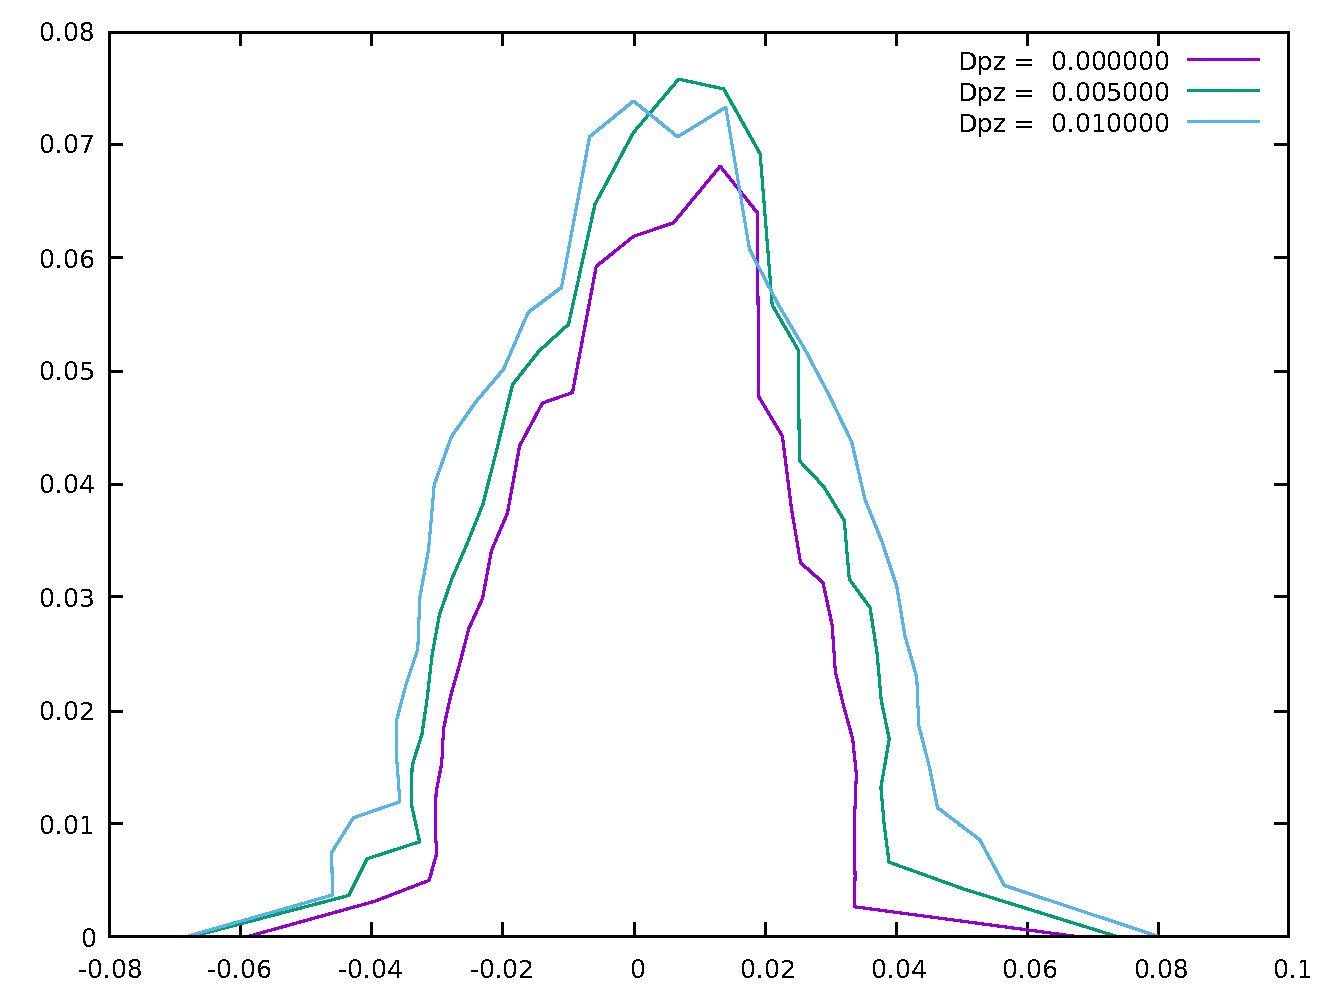
\includegraphics[width=4in]{da-plot.pdf}
  \caption{
Example dynamic aperture plot using \vn{gnuplot}.
  }
  \label{f:da-plot}
\end{figure}

%------------------------------------------------------------------
\Section{Data Output and Plotting}
\label{s:data.out}

The data output file whose name is set by \vn{dat_file} will look like:

\begin{code}
# lat_file              = chess_arc_pretzel_20150106.lat
# set_rf_off            = T
# da_param%min_angle    =  0.0000000
# da_param%max_angle    =  3.1415926
# da_param%rel_accuracy =  1.00E-02
... etc. ...
# da_param%n_angle      = 37
# gnuplot plotting command: 
#   plot for [IDX=1:3] "da.dat" index (IDX-1) u 1:2 w lines ...

"dpz =  0.000000"
"x_ref_orb =  0.000124"
"y_ref_orb =  0.000037"
   0.068125   0.000000    544      Hit +X Side        Q11E
   0.033668   0.002675    442      Hit -Y Side        Q06E
   0.033807   0.005414    717      Hit +Y Side        Q26W
   0.033673   0.008195    410      Hit +X Side        B28W
   0.033759   0.011160    119      Hit -X Side        SEX_08E
   0.034006   0.014403    855      Hit +Y Side        SEX_21W
... etc. ...

dpz =  0.005000"
"x_ref_orb =  0.006591"
"y_ref_orb =  0.006591"
   0.073979   0.000000    904      Hit -Y Side        SEX_16W
   0.050379   0.004234    554      Hit -Y Side        SEX_19E
   0.038989   0.006603    987      Hit -X Side        SEX_39E
   0.038242   0.009842    447      Hit +Y Side        SEX_15W
   0.037746   0.013196    365      Hit +X Side        SEX_41E
... etc. ...
\end{code}

The top part of the data file will be a record of input parameter values. This is followed by a number of
data blocks, one for each setting of \vn{dpz}. The five columns of these data blocks are:
\begin{code}
1 & 2: x_aperture, y_aperture
3:     Number of turns a particle initially at the aperture limit survived. 
4:     Transverse location where particle died.
5:     Lattice element where particle died.
\end{code}
Note that a particle will ``die'' if it hits an aperture or its amplitude is beyond the setting of
\vn{bmad_com%max_aperture_limit}. The default value of this maximum aperture is 1000 meters.

One way to plot the data is to use the \vn{gnuplot} program (documentation for gnuplot is available using a
web search). Run \vn{gnuplot} and use the command printed in the top section of the data file. An example of
what such a plot looks like is shown in Fig.~\ref{f:da-plot}.

%------------------------------------------------------------------
\begin{thebibliography}{9}

\bibitem{b:bmad}
D. Sagan,
``Bmad: A Relativistic Charged Particle Simulation Library''
Nuc.\ Instrum.\ \& Methods Phys.\ Res.\ A, {\bf 558}, pp 356-59 (2006).

\end{thebibliography}

\end{document}

